\documentclass[12pt]{article}
\usepackage[utf8]{inputenc}
\usepackage{ragged2e}
\usepackage{amsmath}
\usepackage{graphicx}
\usepackage{float}
\usepackage{graphicx}
\usepackage{geometry}
\usepackage{setspace}
\usepackage{subcaption}
\geometry{margin=1in}
\setstretch{1.2}
\pagenumbering{gobble}  
\usepackage{chngcntr}

\usepackage{chngcntr}
\counterwithin{figure}{chapter}

\counterwithin{figure}{chapter}
\renewcommand{\thefigure}{\thechapter.\arabic{figure}}

\begin{document}

\begin{center}
\vspace*{1cm}

\textbf{A} \\
\vspace{0.3cm}
\textbf{Major Project} \\
\vspace{0.3cm}
\textbf{Report on} \\[0.5cm]

\textbf{\LARGE Power Quality Disturbance Classification Using Machine Learning} \\[0.5cm]

Submitted in partial fulfilment of the requirements for the \\
curriculum of FY (Sem VI-VIII) \\[0.5cm]


\begin{center}
\begin{tabular}{ll}
\textbf{Allen Salmo Nadar} & \textbf{(1023169)} \\
\textbf{Ryan Norman} & \textbf{(1023170)} \\
\textbf{Tushar Rajendra Patil} & \textbf{(4023126)} \\
\textbf{Sejal Sampat Pawar} & \textbf{(4023128)} \\
\end{tabular}
\end{center}
\vspace{1cm}




Under the Guidance of \\
\textbf{Dr. Bindu S} \\[1cm]


\includegraphics[width=4cm]{logo.png} \\[1cm] 
Department of Electrical Engineering \\
\textbf{Fr. C. Rodrigues Institute of Technology, Vashi} \\

(An Autonomous Institute and Permanently Affiliated to University of Mumbai) \\[0.5cm]

\textbf{2026-27}
\clearpage

\begin{center}
    \vspace{2cm}
    \textbf{\LARGE CERTIFICATE}\\[2cm]
\end{center}
\raggedright
\justifying
 This is to certify that the Major Project entitled "Power Quality Disturbance Classification Using Machine Learning" is a bonafide work of Allen Salmo (1023169),Ryan Norman (1023170), Tushar Rajendra Patil (4023126), Sejal Sampat Pawar (4023128) submitted in partial fulfillment of the requirements for the curriculum of Electrical Engineering FY (Sem VII-VIII) during the academic year 2026-2027.\\[4cm]


\vspace*{2cm}

\begin{center}
\rule{8cm}{0.4pt} \\[0.2cm]
\textbf{Dr. Bindu S} \\[0.2cm]
(Guide)
\end{center}

\vspace{5cm}

\noindent
\begin{minipage}[t]{0.45\textwidth}
\centering
\rule{6cm}{0.4pt} \\[0.2cm]
\textbf{Dr. Mini R} \\[0.2cm]
(Head of Department)
\end{minipage}
\hfill
\begin{minipage}[t]{0.45\textwidth}
\centering
\rule{6cm}{0.4pt} \\[0.2cm]
\textbf{Dr. S.M. Khot} \\[0.2cm]
(Principal)
\end{minipage}
\clearpage

\begin{center}
    \vspace{2cm}
    \textbf{\LARGE Major Project Report Approval}\\[2cm]
\end{center}
\raggedright
\justifying
This Major Project report entitled \textbf{"Power Quality Disturbance Classification Using Machine Learning}is a bonafide work of \textbf{Allen Salmo (1023169),Ryan Norman (1023170), Tushar Rajendra Patil (4023126), Sejal Sampat Pawar (4023128)} is approved for FY Sem VII-VII Electrical Engineering during the academic year 2026-27\\[4cm]


\hspace{10.5cm}\textbf{Examiners:}\\

\raggedleft
1)\rule{5cm}{0.4pt}\\
\vspace{1cm}
2)\rule{5cm}{0.4pt}\\


\raggedright
\vspace{4cm}
\textbf{Date:}\rule{5cm}{0.4pt}\\
\vspace{1cm}
\textbf{Place:}\rule{5cm}{0.4pt}\\
\clearpage

\begin{center}
    \vspace{2cm}
    \textbf{\LARGE Declaration}\\[2cm]
\end{center}

\raggedright
\justifying
We declare that this project report entitled "Power Quality Disturbance Classification Using Machine Learning” represents our ideas in our own words and where others' ideas or words have been
 included, we have adequately cited and referenced the sources. We also declare that we have
 adhered to all principles of academic honesty and integrity and have not misrepresented or
 fabricated or falsified any data/fact in our submission. We understand that any violation of the
 above will be cause for disciplinary action by the Institute and can also evoke penal action
 from the sources which have thus not been properly cited or from whom proper permission
 has not been taken when needed\\[4cm]

\vspace{0cm}

\noindent
\begin{minipage}[t]{0.45\textwidth}
\centering
\rule{6cm}{0.4pt} \\[0.2cm]
\textbf{Allen Salmo Nadar} \\[0.2cm]
(1023169)
\end{minipage}
\hfill
\begin{minipage}[t]{0.45\textwidth}
\centering
\rule{6cm}{0.4pt} \\[0.2cm]
\textbf{Ryan Norman} \\[0.2cm]
(1023170)
\end{minipage}

\vspace{3cm}

\noindent
\begin{minipage}[t]{0.45\textwidth}
\centering
\rule{6cm}{0.4pt} \\[0.2cm]
\textbf{Tushar Rajendra Patil} \\[0.2cm]
(4023126)
\end{minipage}
\hfill
\begin{minipage}[t]{0.45\textwidth}
\centering
\rule{6cm}{0.4pt} \\[0.2cm]
\textbf{Sejal Sampat Pawar } \\[0.2cm]
(4023128)
\end{minipage}
\vspace{1cm}\\
\raggedright
\textbf{Date:}\rule{5cm}{0.4pt}\\\vspace{0.5cm}
\textbf{Place:}\rule{5cm}{0.4pt}

\clearpage

\begin{center}
    \vspace{2cm}
    \textbf{\LARGE Acknowledgment}\\[2cm]
\end{center}

\justifying

I would like to express my deepest gratitude to all those who have contributed to the successful completion of this mini-project, ``Power Quality Disturbance Classification Using Machine Learning.''

\vspace{0.5cm}

Firstly, I am grateful to my guide, Dr. Bindu S, for her valuable guidance, constant encouragement, and support throughout the project. Her insights and advice helped shape the project into its final form.

\vspace{0.5cm}

I extend my heartfelt thanks to Fr. C. Rodrigues Institute of Technology for providing the necessary resources and environment to work on this project. I would also like to acknowledge the assistance of my fellow classmates, whose suggestions and collaboration were of great help during the development process.

\vspace{0.5cm}

Finally, I would like to express my sincere appreciation to my family and friends for their unwavering support and motivation throughout this project.

\vspace{0.5cm}

Thank you all for being a part of this journey.

\clearpage
\begin{center}
    \vspace{2cm}
    \textbf{\LARGE Abstract}\\[2cm]
\end{center}\\
\raggedright
\justifying
Power quality is most  important aspect of modern/smart electrical power systems. In recent years, the use of electronic equipment and nonlinear loads has increased, which can cause different disturbances in the power supply. These disturbances may affect the performance of electrical equipment and reduce the reliability of the system. Therefore, identifying and classifying power quality disturbances is necessary.\\

This project, “Power Quality Disturbance Classification Using Machine Learning,” focuses on simulating different power quality disturbances using MATLAB/Simulink. An IEEE 9-bus power system model is used to study the behaviour of the system under normal and disturbed conditions. Disturbances such as voltage sag, voltage swell, harmonics, interruption, flicker, notch and transient are considered. Voltage and current signals are measured during simulation, and important features such as RMS voltage, peak voltage, total harmonic distortion (THD), crest factor, dominant frequency and disturbance duration are extracted.\\

The collected electrical data is then used for machine learning-based classification, with the aim of identifying the type of disturbance from the extracted features. This approach can help reduce the effort required for manual analysis and support faster identification of power quality problems. The project combines electrical system simulation with data-driven classification to study how machine learning can be applied to power quality monitoring.\\
\clearpage
\begin{center}
    \vspace{2cm}
    \textbf{\LARGE Table Of Content}\\[2cm]
\end{center}\\
\tableofcontents

\clearpage


\begin{center}
    \vspace{2cm}
    \textbf{\LARGE List of Figures}\\[2cm]
\end{center}\\
\listoffigures
\clearpage



\pagenumbering{arabic}
\stepcounter{page}
\begin{center}
    \vspace{2cm}
    \textbf{\LARGE Chapter 1}\\[2cm]
\end{center}\\
\pagenumbering{arabic}
\stepcounter{page}
\section{Introduction}

\subsection{ Introduction}
\raggedright
\justifying
Electrical power systems play an important role in our daily lives, as industries, hospitals, offices and homes depend on a continuous and reliable supply of electricity. However, changes in load, switching operations, faults and nonlinear electrical equipment can affect the normal voltage and current waveforms. Common disturbances include voltage sag, voltage swell, harmonics, interruption, flicker, notch and transient. These conditions can affect the performance of electrical equipment, increase losses and reduce the reliability of the system. Therefore, identifying such disturbances is important for maintaining stable operation.\\

Traditionally, engineers analyse electrical waveforms and use mathematical methods to identify abnormal conditions. Although these methods are useful, analysing large amounts of data manually can take time. Machine learning offers an alternative approach by learning patterns from collected data and using them to classify different conditions. It can help simplify the analysis process and support faster identification of disturbances based on the characteristics of voltage and current signals.\\

This project, Power Quality Disturbance Classification Using Machine Learning, uses an IEEE 9-bus power system model developed in MATLAB/Simulink. Different disturbances are simulated, and the resulting electrical signals are measured to extract features such as RMS voltage, peak voltage, crest factor, total harmonic distortion (THD), dominant frequency and disturbance duration. These features are used to prepare a dataset for machine learning-based classification. The main aim is to identify different disturbance types from the measured parameters and understand how electrical system simulation and machine learning can be combined to improve power system monitoring.\\


\subsection{Motivation}
\raggedright
\justifying
 The increasing use of electronic devices and nonlinear loads has made it more challenging to maintain a stable electricity supply. Disturbances such as voltage sag, swell and harmonics can affect electrical equipment and reduce the overall performance of the power system. This created an interest in understanding how these disturbances occur and how they can be identified.\\

Traditional methods of analysing electrical waveforms may require manual observation and detailed calculations. Studying the application of machine learning provides an opportunity to make the classification process more systematic. By extracting useful features from voltage and current signals, different disturbance types can be identified based on their characteristics.\\

The main motivation behind this project is to combine electrical engineering concepts with machine learning techniques. Using an IEEE 9-bus system in MATLAB/Simulink provides a practical way to simulate different operating conditions and study their effects. The project also helps develop a better understanding of power system behaviour and the use of data-driven methods in electrical monitoring.
\subsection{Aim}
\raggedright
\justifying
The aim of this project is to simulate different power quality disturbances in an IEEE 9-bus power system using MATLAB/Simulink and classify them using machine learning techniques. The project focuses on measuring voltage and current signals, extracting important electrical features, and using these features to identify disturbances such as voltage sag, swell, harmonics, interruption, flicker, notch and transient.

\subsection{Objective}
\raggedright
\justifying
\begin{itemize}
    \item To develop an IEEE 9-bus power system model using MATLAB/Simulink.
\end{itemize}
\begin{itemize}
    \item  To simulate different disturbances, including voltage sag, swell, harmonics, interruption, flicker, notch and transient.
\end{itemize}
\begin{itemize}
    \item  To measure voltage and current signals under normal and disturbed conditions.
\end{itemize}
\begin{itemize}
    \item To extract important electrical features such as RMS voltage, peak voltage, THD and crest factor.
\end{itemize}
\begin{itemize}
    \item To use machine learning techniques to classify different disturbances based on the extracted features.
\end{itemize}


\subsection{Problem Definition}
\raggedright
\justifying
Electrical power systems are affected by various disturbances caused by sudden load changes, switching operations, faults and nonlinear loads. These disturbances change the normal voltage and current waveforms and may affect the performance of electrical equipment. Identifying the type of disturbance can be difficult when several conditions produce similar waveform patterns. Traditional methods often require detailed signal analysis, which can become time-consuming when dealing with large amounts of electrical data.\\

The problem addressed in this project is to develop a systematic method for identifying and classifying different disturbances using machine learning techniques. An IEEE 9-bus system is modelled in MATLAB/Simulink to simulate normal and disturbed operating conditions. Electrical features are extracted from the measured signals and used to prepare a dataset for classification. The objective is to study whether these features can help distinguish between different disturbance types and support efficient analysis of electrical system behaviour.

 
\subsection{Scope}
\raggedright
\justifying
\begin{itemize}
    \item  Modelling an IEEE 9-bus power system using MATLAB/Simulink.
\end{itemize}\begin{itemize}
    \item  Simulating different disturbances, including voltage sag, swell, harmonics, interruption, flicker, notch and transient.
\end{itemize}\begin{itemize}
    \item Measuring and analysing voltage and current signals under different operating conditions.
\end{itemize}\begin{itemize}
    \item  Ensure the system is scalable for various sizes and types of solar installations, both residential and commercial
\end{itemize}\begin{itemize}
    \item Extracting electrical features such as RMS voltage, peak voltage, THD and crest factor.
\end{itemize}\begin{itemize}
    \item  Developing a dataset for machine learning-based disturbance classification.
\end{itemize}\begin{itemize}
    \item Evaluating the classification performance of the trained model using suitable performance metrics.
\end{itemize}\begin{itemize}
    \item  Exploring the future application of the system in power system monitoring and disturbance detection.
\end{itemize}

\clearpage


\begin{center}
    \vspace{2cm}
    \textbf{\LARGE CHAPTER 2}\\[2cm]
\end{center}

\section{Literature review}
This chapter introduces the literature review we have done in making of this project. Many research paper have been study in making of this project. This includes the summary of the literature review 
\subsection{Literature Review}

\begin{itemize}
    \item \textbf{"Classification Methods for Recognition of Power Quality Disturbances in Distribution Networks Using Artificial Neural Network (2023)"}
\end{itemize}
\raggedright
\justifying
This paper presents a method for identifying different electrical disturbances using an Artificial Neural Network (ANN). The researchers use the Discrete Wavelet Transform (DWT) to extract features from simulated signals, which are then used to train the classification model. The method considers disturbances such as voltage sag, swell, harmonics, flicker and transients. The proposed system is implemented in MATLAB/Simulink and tested using an IEEE 9-bus system. The reported classification accuracy is 99.4 percent initially and 95.6 percent during testing on the IEEE 9-bus system. This study is particularly relevant to the present project because it demonstrates the application of machine learning to disturbance classification in a simulated power network.\\

 - Source: W. Buasi and W. Srirattanawichaikul, “Classification Methods for Recognition of Power Quality Disturbances in Distribution Networks Using Artificial Neural Network,” in 2023 IEEE PES 15th Asia-Pacific Power and Energy Engineering Conference (APPEEC), 2023.

DOI: 10.1109/APPEEC57400.2023.10561959
\begin{itemize}
    \item \textbf{Power Quality Disturbance Detection using Machine Learning Algorithm (2020)}
\end{itemize}
   This paper proposes a machine-learning approach for detecting and classifying electrical disturbances using a Decision Tree (DT) classifier. The researchers use a mathematical morphology filter to extract useful features from signals generated through MATLAB-based disturbance models. Ten disturbance categories are considered, including voltage sag, swell, interruption, harmonics, flicker, notch and transient-related events. The extracted features are used to train and test the classifier, and the proposed method reports an accuracy of 99.95 percent. The study highlights the importance of feature extraction and dataset preparation in automated disturbance classification. Its methodology provides a useful reference for developing a classification dataset and selecting suitable features for the present project.\\

 - Source: K. Sekar, S. Sendilkumar, and K. Karthick, “Power Quality Disturbance Detection using Machine Learning Algorithm,” in 2020 IEEE International Conference on Advances and Developments in Electrical and Electronics Engineering (ICADEE), 2020.

DOI: 10.1109/ICADEE51157.2020.9368939

 \begin{itemize}
     \item \textbf{Classification of Power Quality Disturbances Using Machine Learning Methods (2024)}
 \end{itemize}
 This paper investigates the classification of electrical disturbances using different machine-learning algorithms. The researchers apply the Fourier Synchro Squeezing Transform (FSST) to preprocess the signals before classification. Four algorithms are evaluated: Support Vector Machine (SVM), Random Forest (RF), Gradient Boosting Machine (GBM) and Logistic Regression (LR). The reported classification accuracies are 91 percent, 96 percent, 99 percent and 90 percent, respectively, with Gradient Boosting achieving the highest accuracy among the evaluated methods. The study demonstrates that the choice of algorithm can influence classification performance. It is relevant to the present project because it provides a basis for understanding and comparing machine-learning approaches for identifying disturbances from electrical signal data.

 - Source: S. Shivesh, S. V. Ved, N. Reddy K. V., R. Chowdhary I., S. K. G., and R. Satheesh, “Classification of Power Quality Disturbances Using Machine Learning Methods,” in 2024 IEEE 1st International Conference on Green Industrial Electronics and Sustainable Technologies (GIEST), 2024.

DOI: 10.1109/GIEST62955.2024.10959739
 \vspace{1cm}
 

\subsection{Summary of Literature Review and Research Gap}
\raggedright
\justifying
The reviewed research papers present different machine-learning approaches for identifying and classifying electrical disturbances. The first paper uses an Artificial Neural Network (ANN) with Discrete Wavelet Transform (DWT), while the second applies a Decision Tree classifier with mathematical morphology-based feature extraction. The third compares algorithms such as Support Vector Machine (SVM), Random Forest, Gradient Boosting and Logistic Regression. These studies highlight the importance of signal processing, feature extraction and classifier selection in disturbance identification.\\

Research Gap : The reviewed studies use different signal-processing techniques and classification methods, but their approaches do not necessarily match the feature-based method adopted in the present project. There is scope to investigate how electrical features such as RMS voltage, peak voltage, total harmonic distortion (THD), crest factor, dominant frequency and disturbance duration can be used to classify multiple disturbance types in an IEEE 9-bus power system. Therefore, the present project focuses on simulating these conditions in MATLAB/Simulink, extracting relevant electrical features and preparing a dataset for machine-learning-based classification. The effectiveness of this approach will be assessed using the results obtained from the implemented model.

 \clearpage

 
\begin{center}
    \vspace{2cm}
    
   \textbf{\LARGE CHAPTER 3}\\[2cm]
\end{center}


\section{  Proposed System }
 
\subsection{Analysis / Algorithm / Framework }
\vspace{0.5cm}

\justifying
The proposed system focuses on the identification and classification of power quality disturbances using machine learning techniques. An IEEE 9-bus power system is modelled in MATLAB/Simulink to study the behaviour of the network under normal and disturbed operating conditions. The model provides a simulation environment in which different electrical disturbances can be introduced and their effects on voltage and current waveforms can be analysed.\\

The system considers disturbances such as voltage sag, voltage swell, harmonics, interruption, flicker, notch and transient. Each disturbance affects the electrical waveform in a different way. For example, voltage sag reduces the RMS voltage for a short period, while harmonics introduce frequency components other than the fundamental frequency. By simulating these conditions, the corresponding electrical signals can be collected and compared with signals obtained under normal operating conditions.\\

\begin{figure}[H]
    %\centering
    \begin{center}
    
    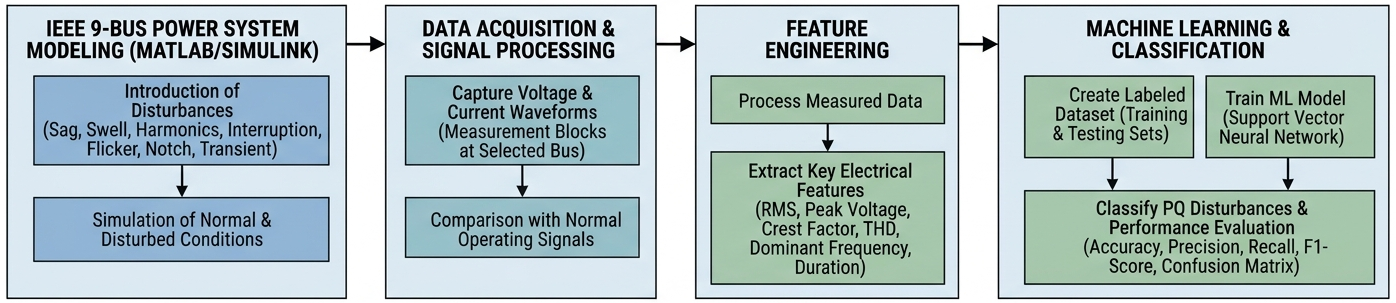
\includegraphics[width=1\textwidth]{block diagram_1.png}
    \caption{High-Level System Architecture}
    \label{fig:High-Level System Architecture}
        
    \end{center}\\
\end{figure}

Voltage and current measurement blocks are used to capture the required signals at the selected bus. The measured data is then processed to extract important electrical features, including RMS voltage, peak voltage, crest factor, total harmonic distortion (THD), dominant frequency and disturbance duration. These features help describe the characteristics of each disturbance and form the input dataset for the machine-learning stage.\\

The dataset is organised using suitable labels for normal operation and each disturbance category. It is then divided into training and testing sets so that the machine-learning model can learn from one portion of the data and be evaluated on unseen samples. The trained model is intended to classify disturbances based on the extracted features. Its performance can be evaluated using metrics such as accuracy, precision, recall, F1-score and a confusion matrix. This framework combines electrical system simulation, signal analysis and machine learning to develop a systematic approach to disturbance classification.\\

\subsection{ Design Methodology}
\justifying The design methodology is divided into several stages, beginning with power system modelling and ending with the evaluation of the classification model.


\begin{enumerate}
    \item Stage 1: Modelling of the IEEE 9-Bus System\\
\justifying The IEEE 9-bus test system is developed in MATLAB/Simulink using generators, transformers, transmission lines, buses and loads. The model represents a power network and provides a base for studying the effect of disturbances on electrical signals. The system is first simulated under normal operating conditions to obtain reference voltage and current waveforms.\\



    \item Stage 2: Simulation of Power Quality Disturbances\\
\justifying
Different disturbance conditions are introduced into the model by applying suitable changes to the electrical system. These include voltage sag, voltage swell, harmonics, interruption, flicker, notch and transient. Each condition is simulated for a specified time interval, and the resulting waveforms are observed. The simulation parameters must be selected carefully so that the generated signals represent the intended disturbance.\\

    \item Stage 3: Measurement and Data Collection\\
    \justifying
    Voltage and current measurement blocks are placed at the selected bus to capture the three-phase electrical signals. The signals are recorded for normal operation and for each simulated disturbance. The collected data provides the basis for further analysis and helps identify how the electrical parameters change under different conditions.\\

\begin{figure}[H]
    %\centering
    \begin{center}
    
    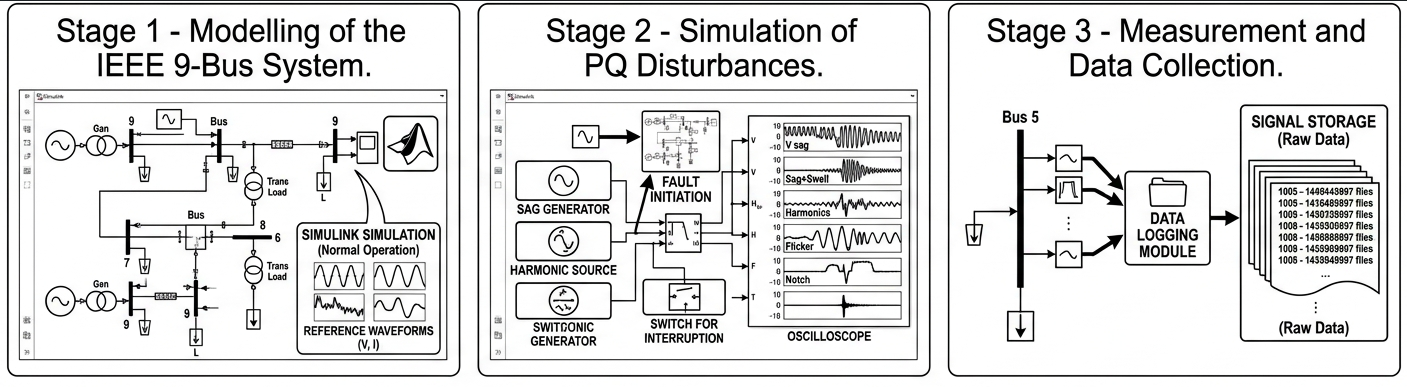
\includegraphics[width=1\textwidth]{step1_3.png}
    \caption{Power System Simulation and Raw Signal Measurement Phase}
    \label{fig:Power System Simulation and Raw Signal Measurement Phase}
        
    \end{center}\\
\end{figure}

   \item Stage 4: Feature Extraction and Dataset Preparation\\
   \justifying
   The recorded signals are processed to calculate relevant features such as RMS voltage, peak voltage, crest factor, THD, dominant frequency and disturbance duration. These parameters are arranged in a structured dataset, with each sample assigned the appropriate disturbance label. The dataset is checked for missing values, incorrect labels and inconsistent measurements before being used for model development.\\


    \item Stage 5: Machine-Learning Model Development\\
    \justifying
    The prepared dataset is used to train a suitable machine-learning classifier. During training, the model learns the relationship between the extracted electrical features and the corresponding disturbance categories. The dataset is divided into training and testing portions to evaluate how well the model classifies samples that were not used during training. The selected algorithm and its parameters can be adjusted based on the observed results.\\



    \item Stage 6: Testing and Performance Evaluation\\
    \justifying
    The trained model is tested using unseen data, and its predicted disturbance labels are compared with the actual labels. Performance metrics such as accuracy, precision, recall and F1-score are calculated to understand the model's classification capability. A confusion matrix can also be used to identify which disturbance types are classified correctly and which are confused with one another. The results are then analysed to determine the strengths and limitations of the proposed system.\\

\begin{figure}[H]
    %\centering
    \begin{center}
    
    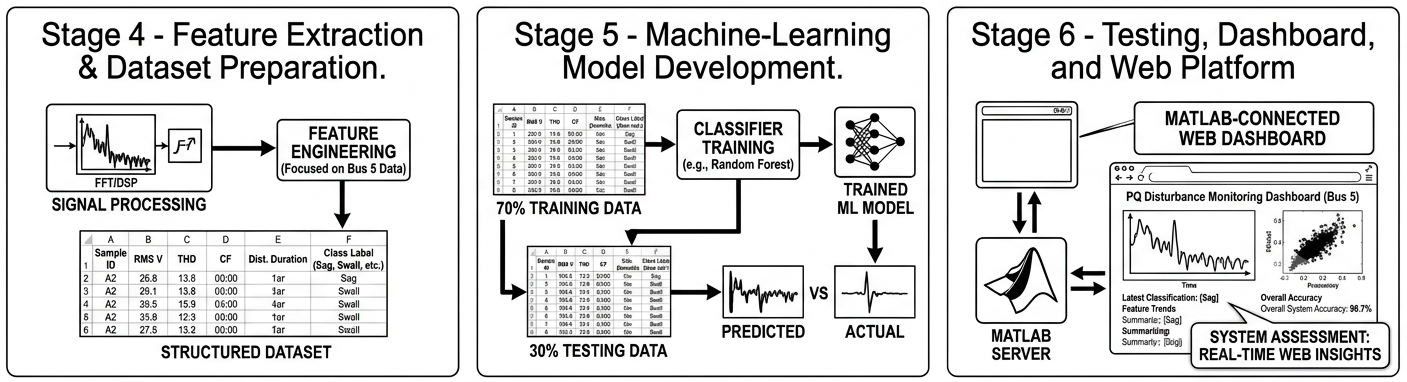
\includegraphics[width=1\textwidth]{step4_6.png}
    \caption{Machine Learning Workflow}
    \label{fig:Machine Learning Workflow}
        
    \end{center}\\
\end{figure}


Through these stages, the proposed methodology establishes a link between power system simulation and machine-learning-based analysis. It provides a structured way to study different disturbances, prepare electrical data and evaluate the ability of a classifier to distinguish between normal and abnormal operating conditions.
\clearpage\\

\begin{center}
    \vspace{2cm}
    \textbf{\LARGE CHAPTER 4}\\[2cm]
\end{center}

\section{Experimental Setup}

\subsection{Input Data / Dataset Details}

\justifying
The input data for this project is generated by simulating an IEEE 9-bus power system in MATLAB/Simulink. The model is used to study normal operating conditions and different power quality disturbances. The disturbances considered include voltage sag, voltage swell, harmonics, interruption, flicker, notch and transient. Voltage and current signals are measured at the selected bus during the simulation, and the recorded signals are used for further analysis.\\

The collected signals are processed to extract important electrical features, such as RMS voltage, peak voltage, crest factor, total harmonic distortion (THD), dominant frequency and disturbance duration. These features are arranged in a structured dataset, with each sample assigned a corresponding label. The labels represent normal operation and the different disturbance categories. The dataset is intended for training and testing a machine-learning model to identify the type of disturbance based on the extracted electrical parameters.\\

\subsection{Software and Hardware Specifications}
\justifying
The project primarily uses MATLAB/Simulink for power system modelling, disturbance simulation and electrical signal analysis. MATLAB is also used to process the collected signals, calculate the required features and prepare the dataset. A suitable machine-learning environment, such as MATLAB or Python, can be used for model training and evaluation, depending on the implementation adopted for the project.
-
\justifying
\begin{itemize}
    \item  MATLAB: For numerical calculations, signal processing and feature extraction.
\end{itemize}\begin{itemize}
    \item Simulink: For modelling and simulating the IEEE 9-bus power system.
\end{itemize}\begin{itemize}
    \item Simscape Electrical / Specialized Power Systems: For representing electrical components and analysing system behaviour, where applicable.
\end{itemize}\begin{itemize}
    \item Machine-learning tools: MATLAB Machine Learning Toolbox or Python libraries such as Scikit-learn, depending on the classifier implementation.
\end{itemize}\\\vspace{1cm}



\begin{figure}[H]
    %\centering
    \begin{center}
    
    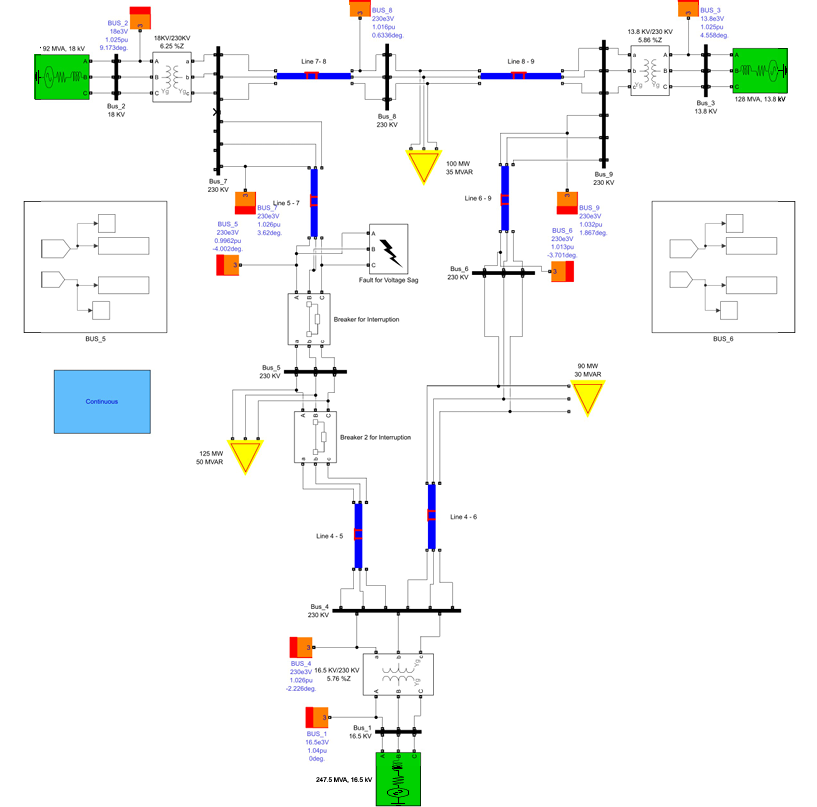
\includegraphics[width=1\textwidth]{simulation.png}
    \caption{IEEE 9 Bus System}
    \label{fig:IEEE 9 Bus System}
        
    \end{center}\\
\end{figure}

\clearpage

\subsection{Evaluation Parameters}

\justifying
The performance of the proposed system is evaluated by examining the extracted electrical features and the classification results obtained from the machine-learning model. The electrical parameters help describe the characteristics of the simulated disturbances, while classification metrics measure how effectively the model identifies each disturbance category.\\

The main electrical features used for analysis are:

\justifying
\begin{itemize}
    \item  RMS Voltage: Represents the effective value of the measured voltage and helps identify voltage sag and swell.
\end{itemize}\begin{itemize}
    \item Peak Voltage: Indicates the maximum magnitude of the waveform during the observation period.
\end{itemize}\begin{itemize}
    \item Total Harmonic Distortion (THD): Measures waveform distortion caused by harmonic components
\end{itemize}\begin{itemize}
    \item Disturbance Duration: Measures the time interval over which a disturbance occurs..
\end{itemize}

The machine-learning model can be evaluated using the following performance metrics: 
\justifying
\begin{itemize}
    \item  Accuracy: Measures the proportion of correctly classified samples.
\end{itemize}\begin{itemize}
    \item Precision: Indicates how many samples predicted as a particular disturbance actually belong to that category.
\end{itemize}
\clearpage

\begin{center}
    \vspace{1.5cm}
    \textbf{\LARGE CHAPTER 4}\\[1.5cm]
\end{center}
\section{Result}\\
\subsection{Result and Discussion}

\raggedright
\justifying
The IEEE 9-bus power system was modelled in MATLAB/Simulink to study the behaviour of the electrical network under normal operating conditions and during different power quality disturbances. The simulation provides a way to observe changes in voltage and current waveforms when disturbances are introduced. Each disturbance produces different changes in the electrical signals, which can be analysed to understand its effect on the system.\\

The simulated signals are used to extract electrical features such as RMS voltage, peak voltage, crest factor, total harmonic distortion (THD), dominant frequency and disturbance duration. These parameters help distinguish normal operation from disturbed conditions. For example, voltage sag is associated with a reduction in RMS voltage, while voltage swell produces an increase. Harmonics introduce additional frequency components into the waveform, resulting in distortion of the normal sinusoidal shape. Similarly, interruption, flicker, notch and transient produce different waveform characteristics that can be studied through signal analysis.\\

The extracted features are organised into a dataset for machine-learning-based classification. This dataset provides the basis for training and testing the classification model to identify different disturbance categories. The model's performance can be examined using metrics such as accuracy, precision. These measures help determine how effectively the model distinguishes between disturbance types and identify cases where similar signal characteristics may lead to incorrect classification.

Overall, the proposed approach combines electrical system simulation, feature extraction and machine learning to study the classification of power quality disturbances. It provides a systematic method for analysing simulated electrical signals and understanding the potential application of machine learning in power system monitoring. The final conclusions regarding classification accuracy and effectiveness should be based on the actual simulation outputs and model evaluation results.\\




\clearpage



\begin{center}
    \vspace{2cm}
    \textbf{\LARGE CHAPTER 5}\\[1cm]
\end{center}\\



\section{Conclusion and Future Scope}\\
\subsection{Conclusion}
\raggedright
\justifying
The project, Power Quality Disturbance Classification Using Machine Learning, focuses on studying different electrical disturbances through simulation and data analysis. An IEEE 9-bus power system is modelled in MATLAB/Simulink to observe the behaviour of the network under normal and disturbed operating conditions. Disturbances such as voltage sag, voltage swell, harmonics, interruption, flicker, notch and transient are considered for analysis.

Voltage and current signals obtained from the simulations are used to extract important electrical features, including RMS voltage, peak voltage, crest factor, total harmonic distortion (THD), dominant frequency and disturbance duration. These features form the basis for preparing a dataset for machine-learning-based classification. The project provides an understanding of how electrical system simulation and machine learning can be combined to analyse and identify different disturbance types. The effectiveness of the classification approach can be determined through the results obtained from model testing and evaluation.

\subsection{Future Scope}\\
\justifying The project can be extended in several ways to improve its classification capability and practical application.
\justifying
\begin{itemize}
    \item  Improved Classification: Different machine-learning algorithms can be tested and compared to identify the most suitable model for the selected disturbance categories.
\end{itemize}\begin{itemize}
    \item Additional Disturbances: More complex events and combinations of disturbances can be included to study their effects on electrical waveforms.
\end{itemize}
\begin{itemize}
    \item Enhanced Feature Extraction: Additional signal-processing techniques can be explored to improve the distinction between disturbances with similar characteristics.
\end{itemize}\begin{itemize}
    \item Real-Time Monitoring: The simulation-based approach can be extended towards real-time analysis using suitable measurement and data-acquisition systems.
\end{itemize}
\begin{itemize}
    \item  Hardware Implementation: In future work, the trained model could be tested with measured electrical signals or a suitable low-voltage experimental setup.
\end{itemize}\begin{itemize}
    \item Integration with Smart Grids: The approach could be further investigated for use in smart-grid monitoring systems to support disturbance identification and power quality analysis.
\end{itemize}

\clearpage

\begin{center}
    \vspace{2cm}
    \textbf{\LARGE References}\\[2cm]
\end{center}
\section{ References}
\begin{enumerate}
\item W. Buasi and W. Srirattanawichaikul, “Classification Methods for Recognition of Power Quality Disturbances in Distribution Networks Using Artificial Neural Network,” in 2023 IEEE PES 15th Asia-Pacific Power and Energy Engineering Conference (APPEEC), 2023. doi: 10.1109/APPEEC57400.2023.10561959.\\

\item“Power Quality Disturbance Detection using Machine Learning Algorithm,” in 2020 IEEE International Conference on Advances and Developments in Electrical and Electronics Engineering (ICADEE), 2020. doi: 10.1109/ICADEE51157.2020.9368939.\\

\item “Classification of Power Quality Disturbances Using Machine Learning Methods,” in 2024 IEEE 1st International Conference on Green Industrial Electronics and Sustainable Technologies (GIEST), 2024. doi: 10.1109/GIEST62955.2024.10959739.\\




\end{enumerate}

\end{document}




